\subsection{Image Capture Reliability}
\label{sec:release-process}

The Samsung camera software is a privileged system application whose image-capture workflow spans multiple system-level components across the Android software stack.
Consequently, capture failures discovered late in the release cycle may require firmware-level changes involving cross-component coordination and extensive revalidation.
To detect capture failures early, the latest development builds are automatically tested each day across camera workflows, device models, and OS versions.
In addition to this daily testing, the camera-validation team and development engineers periodically stress-test the latest builds to identify timing- and memory-related failures, diagnose their root causes, and verify fixes.
Together, these activities form the core validation process for capture reliability.

A key reliability criterion in this validation process is a fixed internal deadline, referred to as the \emph{Capture Timeout}.
For each capture request, the timeout clock starts when the framework accepts the request, and the draft sequence must produce an initial user-visible image, called the \emph{draft image}, before the deadline.
If the draft sequence fails to produce the draft image within this deadline, the application intentionally crashes to make the violation observable.
Identifying and resolving such violations is therefore an important part of Samsung's pre-release validation process.

% Notes: docs/exhibits.md#fig_draft_final_gap
\begin{figure}[!ht]
  \centering
  \setlength{\tabcolsep}{1pt}%
  % All views are the same 1:1 frame (1080 bp source);
  % the zoom box keeps the source region x 162--702, y 695--875 bp from the bottom.
  % TODO: Replace the middle panel and its crop with the actual draft image
  % produced by lightweight multi-frame composition. Both temporarily reuse
  % fig_draft_final_gap_final.jpg; the caption explicitly marks this placeholder.
  \begin{tabular}{@{}ccc@{}}
    \begin{tikzpicture}
      \node[inner sep=0, anchor=south west] (im) at (0,0)
        {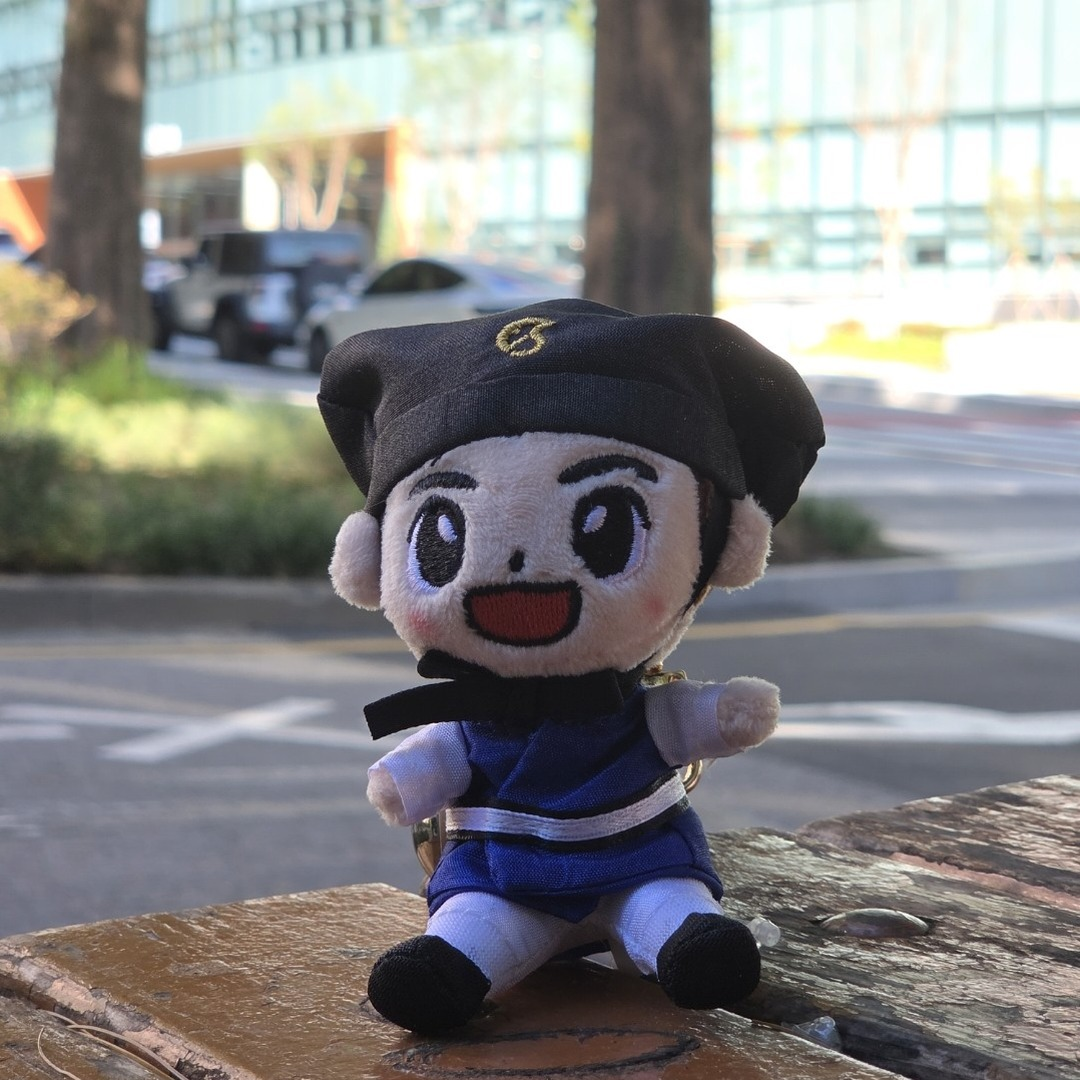
\includegraphics[width=0.325\columnwidth]{figures/fig_draft_final_gap_draft.jpg}};
      \begin{scope}[x={(im.south east)}, y={(im.north west)}]
        \draw[orange, line width=0.8pt] (0.15,0.6435) rectangle (0.65,0.8102);
      \end{scope}
    \end{tikzpicture} &
    \begin{tikzpicture}
      \node[inner sep=0, anchor=south west] (im) at (0,0)
        {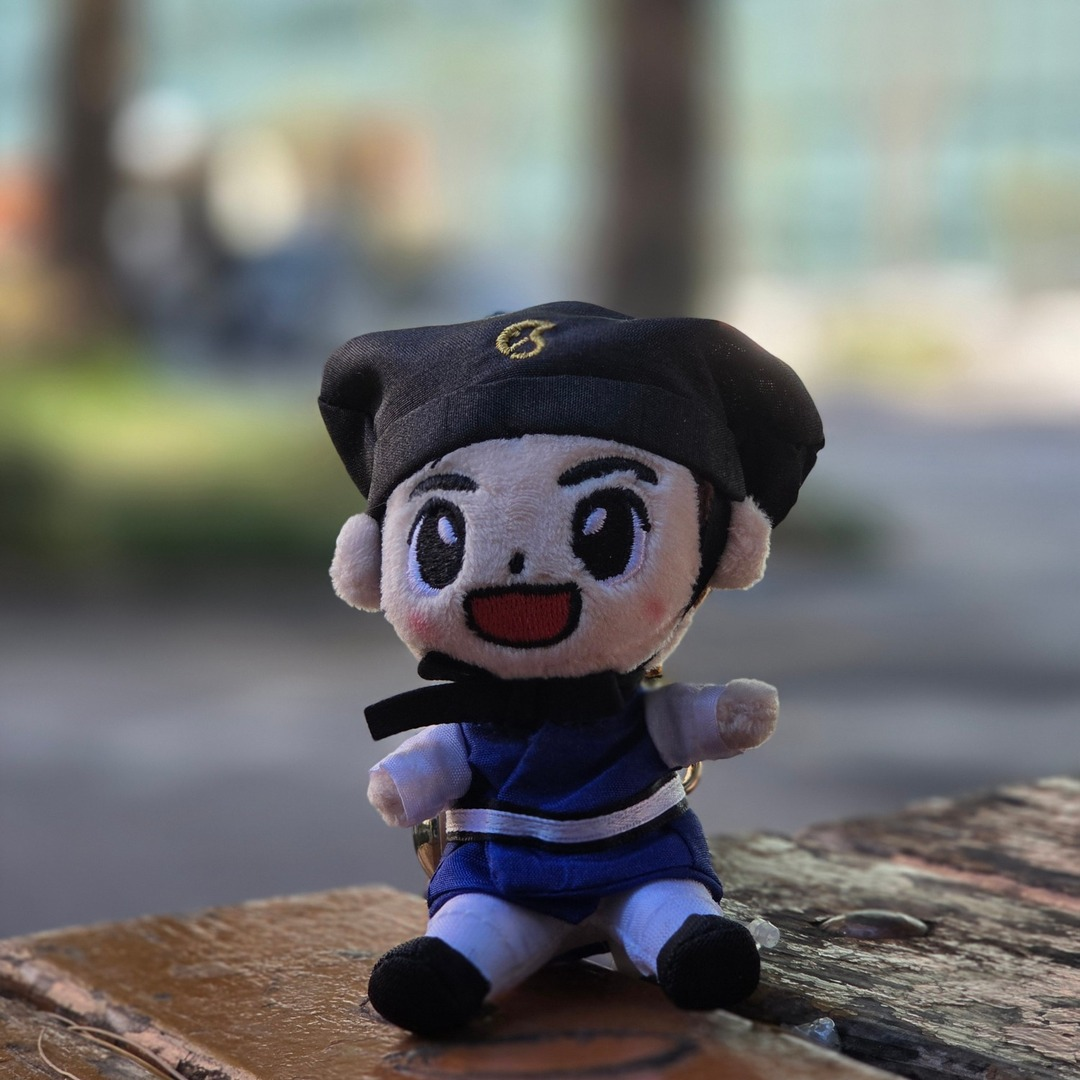
\includegraphics[width=0.325\columnwidth]{figures/fig_draft_final_gap_final.jpg}};
      \begin{scope}[x={(im.south east)}, y={(im.north west)}]
        \draw[orange, line width=0.8pt] (0.15,0.6435) rectangle (0.65,0.8102);
      \end{scope}
    \end{tikzpicture} &
    \begin{tikzpicture}
      \node[inner sep=0, anchor=south west] (im) at (0,0)
        {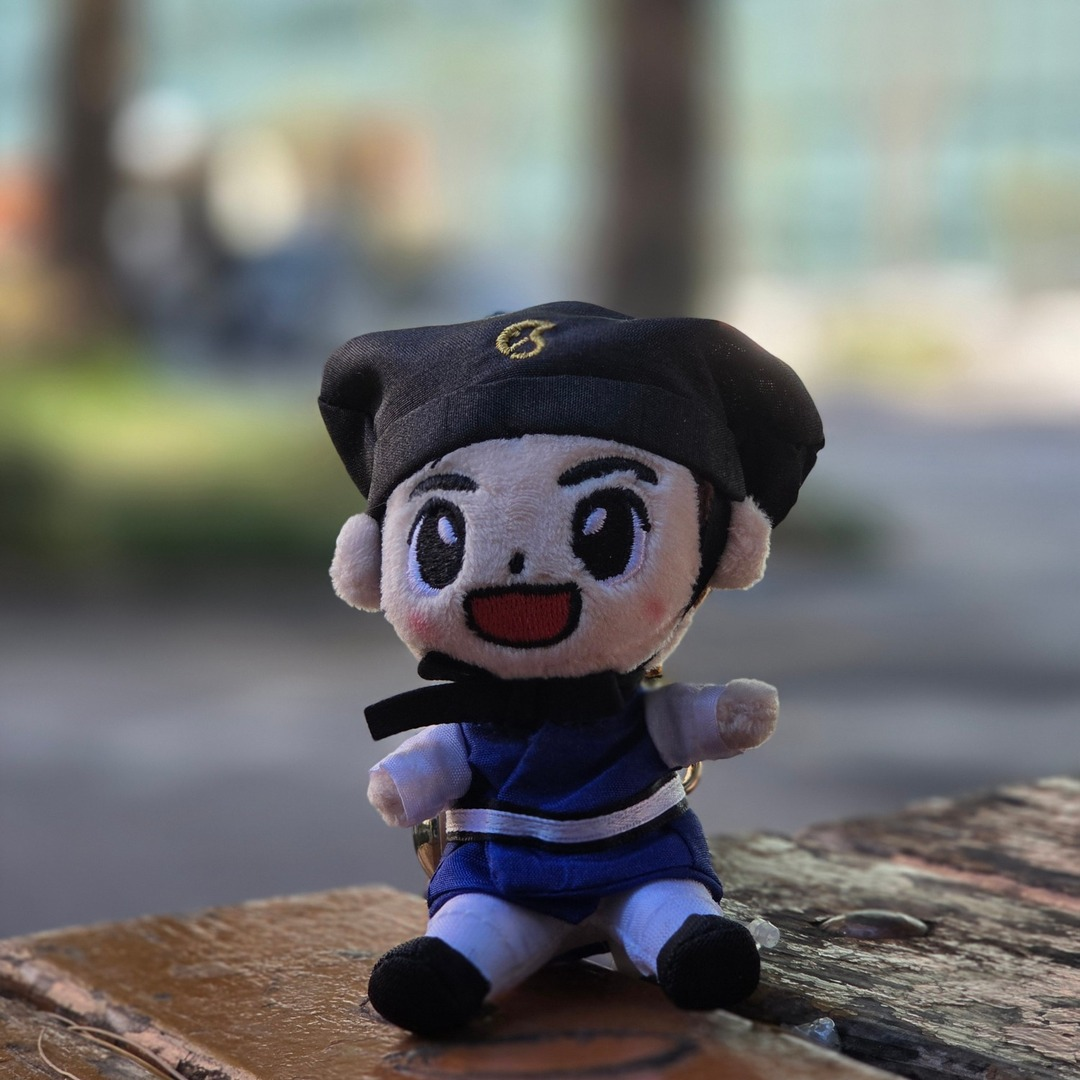
\includegraphics[width=0.325\columnwidth]{figures/fig_draft_final_gap_final.jpg}};
      \begin{scope}[x={(im.south east)}, y={(im.north west)}]
        \draw[orange, line width=0.8pt] (0.15,0.6435) rectangle (0.65,0.8102);
      \end{scope}
    \end{tikzpicture} \tabularnewline[1pt]
    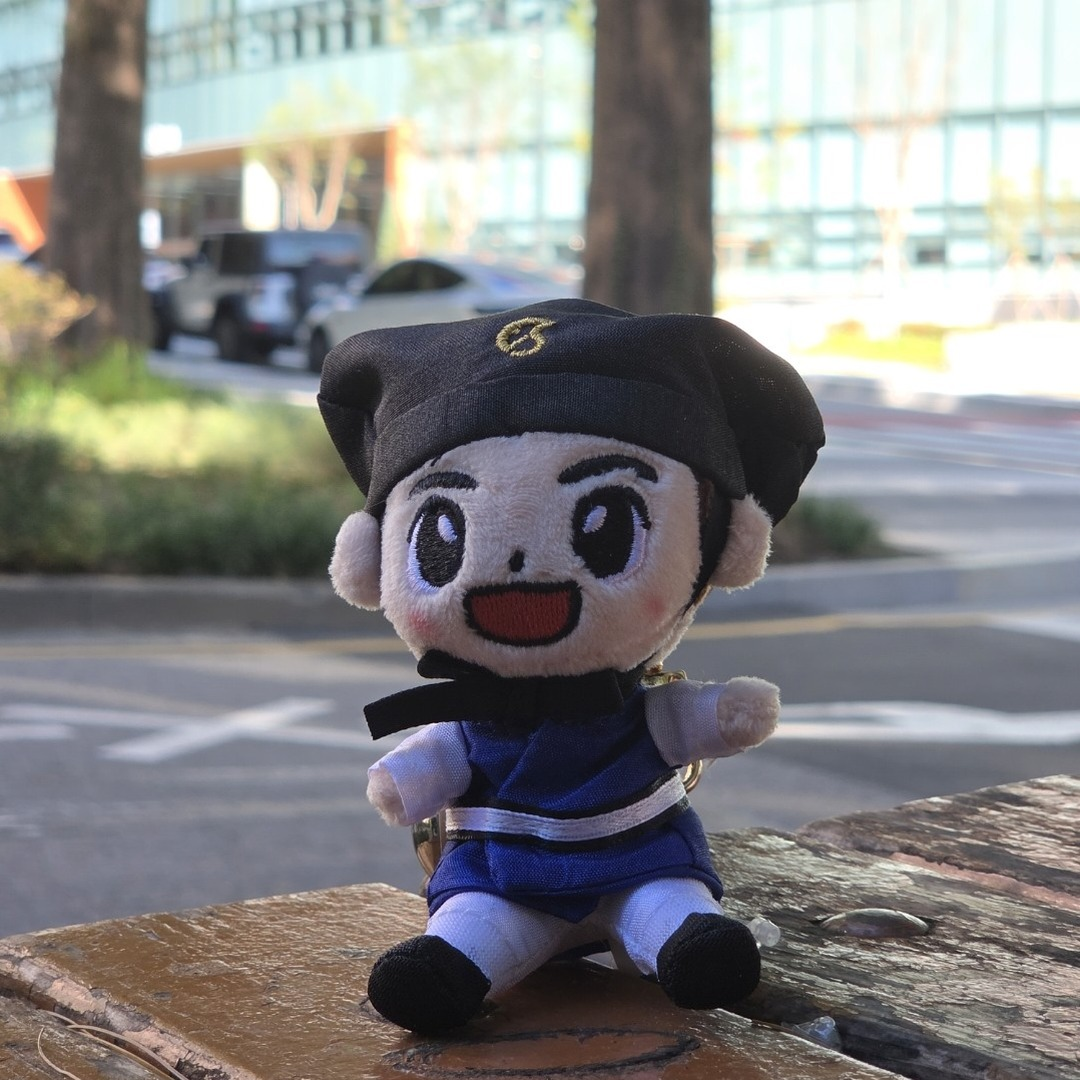
\includegraphics[width=0.325\columnwidth, trim=162 695 378 205, clip]{figures/fig_draft_final_gap_draft.jpg} &
    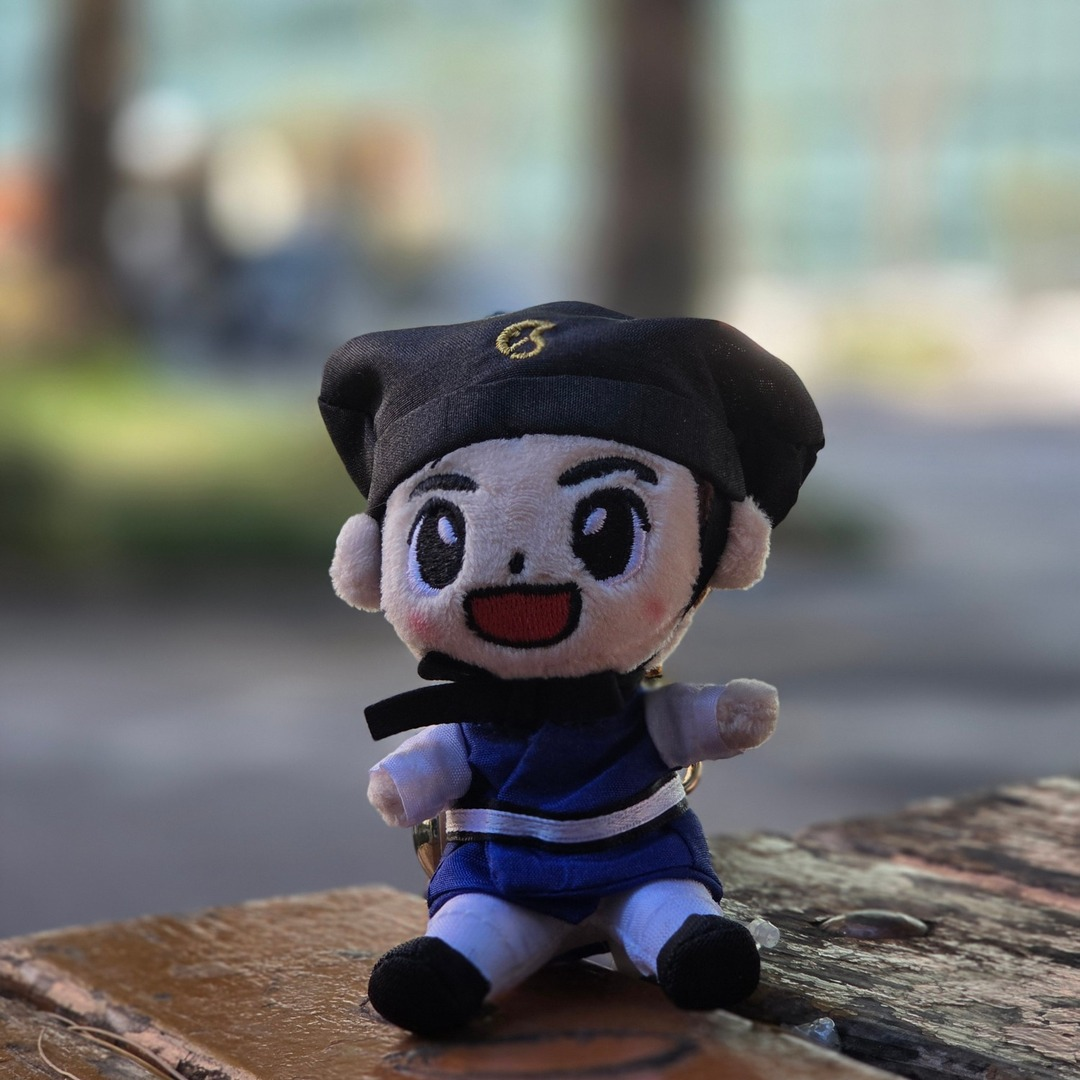
\includegraphics[width=0.325\columnwidth, trim=162 695 378 205, clip]{figures/fig_draft_final_gap_final.jpg} &
    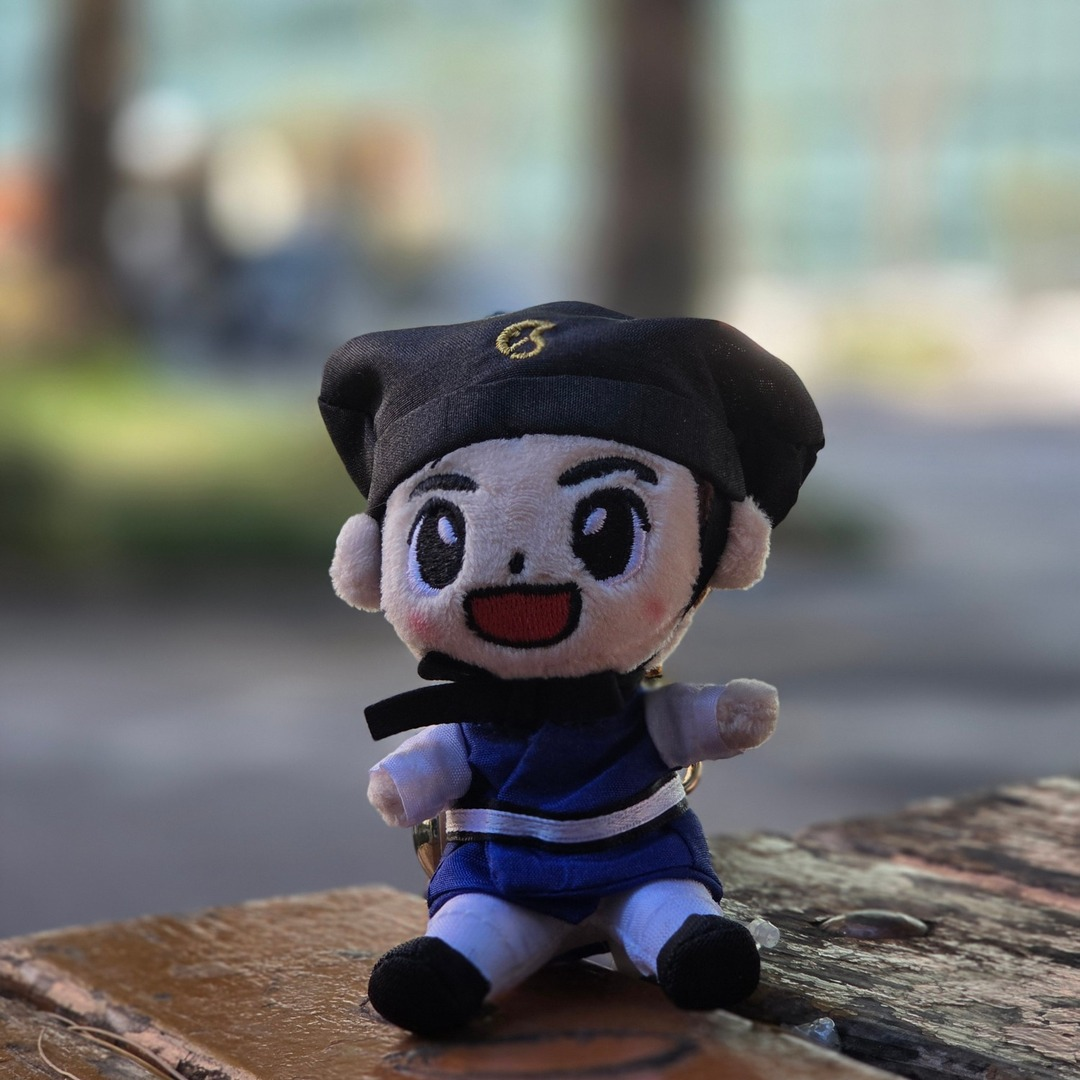
\includegraphics[width=0.325\columnwidth, trim=162 695 378 205, clip]{figures/fig_draft_final_gap_final.jpg}
    \tabularnewline[2pt]
    \parbox[t]{0.325\columnwidth}{\centering\scriptsize (a) Draft image} &
    \makebox[0.325\columnwidth][c]{%
      \parbox[t]{0.41\columnwidth}{\centering\scriptsize
        (b) Draft image with \\lightweight multi-frame composition}} &
    \parbox[t]{0.325\columnwidth}{\centering\scriptsize (c) Final image}
  \end{tabular}
  \caption{Draft--final visual differences in Portrait mode.}
  \label{fig:draft-final-gap}
\end{figure}



\subsection{Camera Usability}
\label{sec:camera-usability}
\label{sec:draft-background}

To enhance camera usability, Samsung aims to provide users with draft images as quickly as possible, support rapid consecutive captures, and minimize the visual difference between draft and final images.
To achieve these goals, Samsung employs a draft sequence, parallel capture, and lightweight multi-frame composition, respectively.

\myparagraph{Draft Sequence}
The draft sequence produces a draft image that users can view before computationally intensive post-processing generates the final image.
Once post-processing completes, the final image replaces the draft image.
To maintain responsiveness, Samsung delays final image generation until the camera application moves to the background in certain shot modes.
Consequently, users may view the draft image for an extended period, making it important to minimize the visual difference between draft and final images.

\myparagraph{Parallel Capture}
Parallel capture reduces the shot-to-shot interval by allowing a new capture request to be accepted before the preceding capture produces its draft image.
This is enabled by a capture-availability signal, \texttt{captureAvailable}, sent from the hardware abstraction layer (HAL) through the camera framework to the application.
By allowing consecutive captures to overlap, parallel capture enables users to take multiple photos in quick succession.

\myparagraph{Lightweight Multi-Frame Composition}
To reduce the visual difference between draft and final images, Samsung developed lightweight multi-frame composition (MFC) for the draft sequence.
MFC combines information from multiple captured frames to improve the draft image before it is displayed to users.
This difference is particularly noticeable in Portrait mode, where the background remains relatively sharp in the original draft image (Figure~\ref{fig:draft-final-gap}(a)), whereas it is blurred in the final image (Figure~\ref{fig:draft-final-gap}(c)).
With MFC, the draft image (Figure~\ref{fig:draft-final-gap}(b)) exhibits background blur that more closely resembles the final image.




\iffalse

\subsection{Capture Reliability}
\label{sec:release-process}
The Samsung camera software is a privileged system application whose image-capture workflow spans multiple system-level components across the Android software stack.
Consequently, capture failures discovered late in the release cycle may require firmware-level changes involving cross-component coordination and extensive revalidation.
To detect capture failures early, the latest development builds are automatically tested each day across camera workflows, device models, and OS versions.
In addition to this daily testing, the camera-validation team and development engineers periodically stress-test the latest builds to identify timing- and memory-related failures, diagnose their root causes, and verify fixes.
Together, these activities form the core validation process for capture reliability.

\myparagraph{Capture Timeout}
A key reliability criterion in this validation process is a fixed internal deadline, referred to as the \emph{Capture Timeout}.
For each capture request, the timeout clock starts at request acceptance, and the ``draft sequence" must produce an initial user-visible draft image before the deadline.
A timeout violation intentionally crashes the application, making the failure immediately observable during testing.
Any such violation blocks the release until developers address its root cause or restrict the affected feature under the conditions that trigger the violation.
Therefore, identifying and resolving Capture Timeout violations is an important reliability task in Samsung's camera development process.
\fi